% todo: mencionar Hofmeister
% todo: revisar esta parte, deixar ela meio que um ``resumo'' do mínimo necessário para se saber sobre a tese.
% todo: citar a classificação da Cécile em vários tipos de micelas que podem ser formadas, tese Danila

\part{Introdução}
	\chapter{Surfactantes e autoassociação}
	
	Surfactantes são moléculas anfifílicas, ou seja, possuem regiões com polaridades diferentes. Uma das regiões interage com com o solvente, e portanto é chamada de liofílica, e a outra interage mal, chamada de liofóbica. Quando o solvente é água, essas regiões são chamadas então hidrofílicas e hidrofóbicas, respectivamente. Essas diferenças de afinidade resultam na orientação das moléculas de surfactante de acordo com as moléculas ao redor, de maneira a maximizar a quantidade de interações favoráveis. A figura \ref{fig:estrutura_surfactantes} mostra a estrutura de alguns surfactantes.
	
	\begin{figure}[H]  % todo: aumentar o tamanho das letras nessa figura
		\centering
		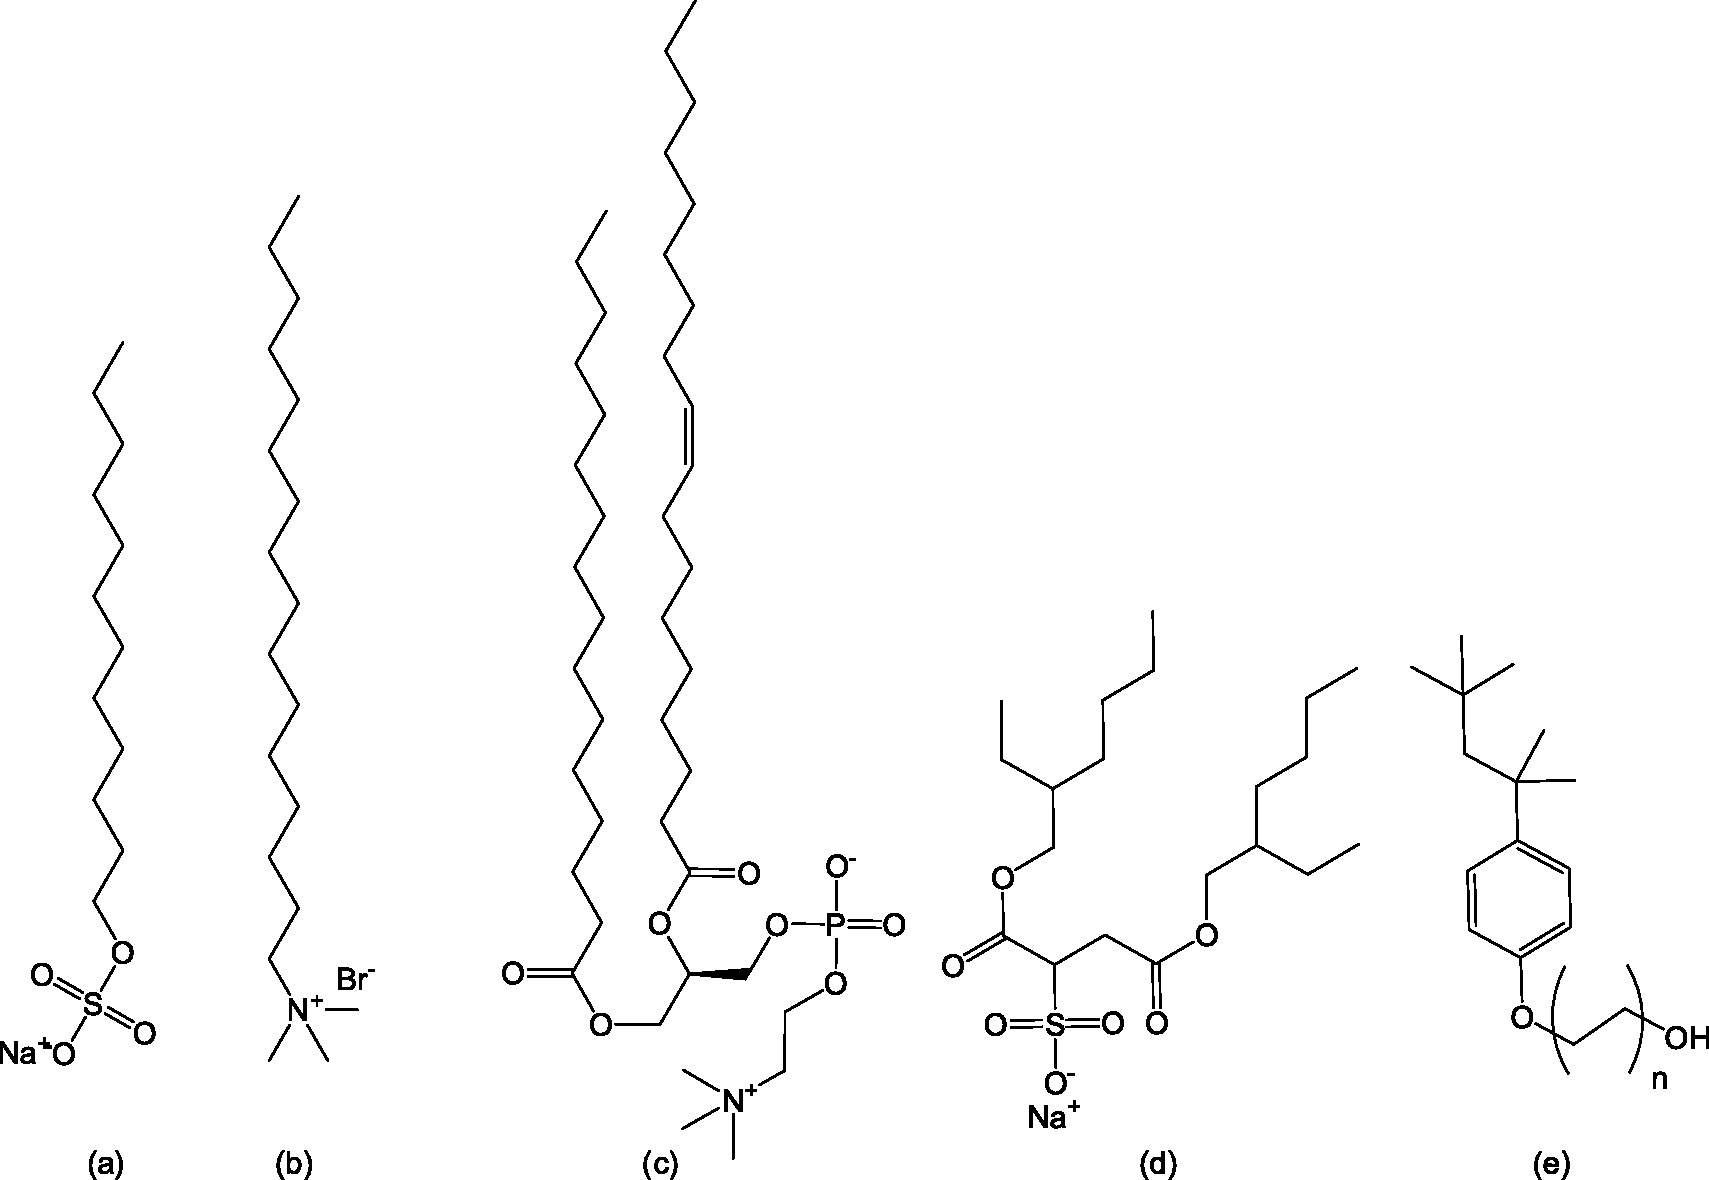
\includegraphics[width=6cm]{./imagens/introducao/estrutura_surfactantes}
		\caption{Estruturas de alguns surfactantes. (a) dodecilsulfato de sódio (SDS) (b) brometo de hexadeciltrimetilamônio (\CTAB) (c) 1-palmitoil-2-oleoil-3-sn-fosfatidilcolina (d) bis-(2-etilhexil) sulfosuccinato de sódio (AOT) (e) poli(etilenoglicol) p-(1,1,3,3-tetrametilbutil)-fenil éter (Triton X-100)}
		\label{fig:estrutura_surfactantes}
	\end{figure}
	
	Em solução aquosa, as moléculas de surfactante se orientam na interface com o ar, com a região apolar direcionada para o ar, e a região polar direcionada para a água (Fig. \ref{fig:superficie_surfactante}. Esse efeito está relacionado à maior favorabilidade das interações polares com a água. É necessário, entretanto, considerar também as moléculas de solvente. Para maximizar as ligações de hidrogênio, as moléculas de água devem se organizar ao redor da cadeia hidrofóbica, resultando numa perda alta de entropia. Caso essas moléculas de água sejam liberadas, por exemplo, orientando a região apolar para o ar, o ganho entrópico das moléculas de água se sobrepõe à perda entrópica das moléculas de surfactante. Esse efeito, conhecido como efeito hidrofóbico, é um força motriz bastante importante da química coloidal.
	
	\begin{figure}
		\centering
		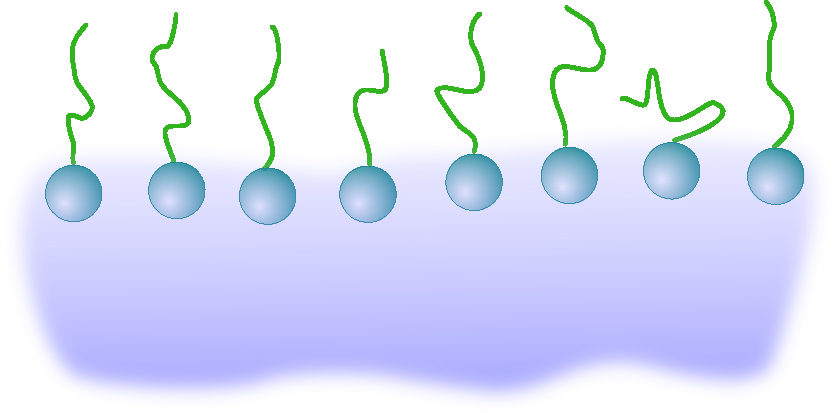
\includegraphics[width=0.7\textwidth]{./imagens/introducao/superficie_surfactante}
		\caption{Interface de água e ar, com moléculas de surfactantes direcionadas}
		\label{fig:superficie_surfactante}
	\end{figure}
	
	À medida que mais surfactante é adicionado, mais moléculas se concentram na superfície, até uma concentração limite. Nessa concentração, chamada de concentração micelar crítica (\cmc) as moléculas começam a formar estruturas de autoassociação, como, por exemplo, micelas esféricas (Fig. \ref{fig:micela_esferica}). Da mesma forma que no caso das moléculas de surfactante na superfície, a perda entrópica da formação de micelas é compensada pelo ganho entrópico das moléculas de água. 
	
	% todo: verificar bem os casos onde isso acontece.
	% todo: pensar se eu devo ilustrar o efeito hidrofóbico
	
	\begin{figure}[H]
		\centering
		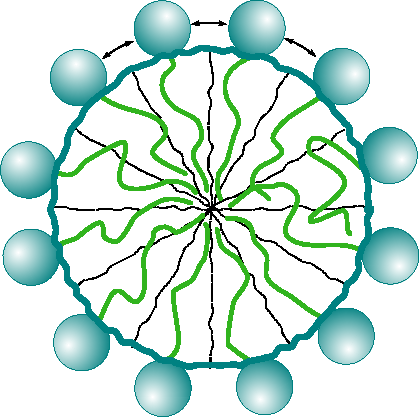
\includegraphics[width=5cm]{./imagens/introducao/micela_esferica}
		\caption{Micela esférica formada por surfactantes em água}
		\label{fig:micela_esferica}
	\end{figure}
	
	Outras estruturas de autoassociação, além de micelas esféricas, são possíveis. Micelas esféricas podem se deformar, gerando micelas esferoidais, podendo possuir até 3 raios diferentes. Após isso, as micelas podem crescer unidimensionalmente, formando micelas cilíndricas. Esse crescimento pode continuar, formando micelas que possuem uma variedade de nomes na literatura, como vermiformes (\emph{wormlike}), gigantes (\emph{giant}), alongadas (\emph{elongated}), filiformes (\emph{threadlike}), parecidas com polímeros (\emph{polymerlike}). Os nomes mais comuns são \emph{wormlike} em inglês e \emph{gigantes} em português. As micelas gigantes são o foco deste trabalho. Uma ilustração de micelas gigantes se encontra na Fig. \ref{fig:micela_gigante}.
		
	% todo: colocar citações com exemplos desses nomes
	% todo: colocar uma figura com um desenho de micelas gigantes
	
	\begin{figure}[H]
		\centering
		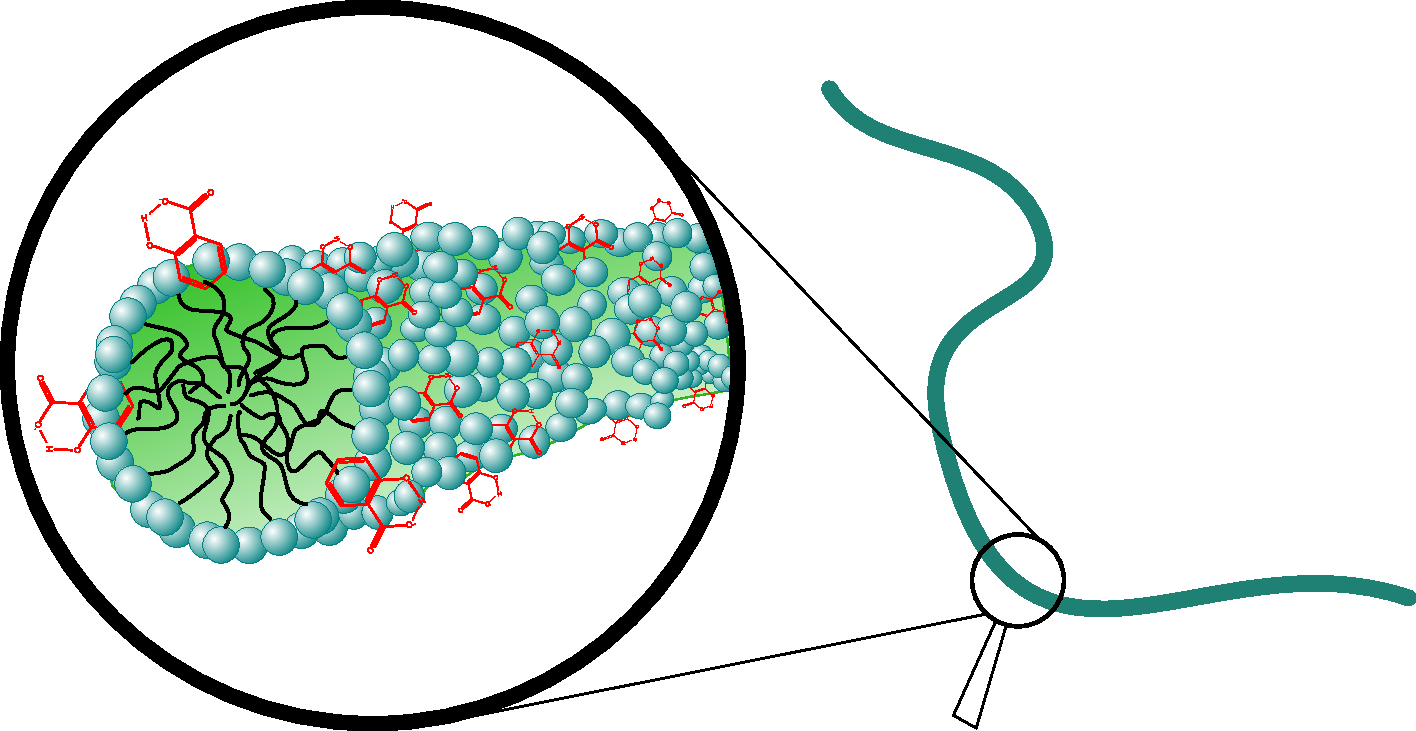
\includegraphics[width=0.7\textwidth]{./imagens/introducao/micela_gigante}
		\caption{Micela gigante formada pela interação de salicilato de sódio e brometo de hexadeciltrimetilamônio}
		\label{fig:micela_gigante}
	\end{figure}
	
	Continuando a adição de surfactante, é possível a formação de várias outras estruturas de autoassociação. O fator que diferencia essas estruturas é o empacotamento da molécula de surfactante, que acaba resultando em curvaturas diferentes. O parâmetro de empacotamento \(P\) (Eq. \ref{eqn:param_empacot}) é um parâmetro geométrico utilizado para racionalizar o empacotamento das moléculas de surfactante.
	
	\begin{equation}
		P = \dfrac{\sfrac{V\!}{l}}{a_0}
		\label{eqn:param_empacot}
	\end{equation}
	
	% todo: colocar a figura do param. de empacot.
	% todo: nicefrac?
	\noindent onde \(V\) é o volume da cadeia hidrofóbica, \(l\) é o comprimento da mesma e \(a_0\) é a área da região polar do surfactante. A figura \ref{fig:param_empacotamento} ilustra os elementos que compõem o parâmetro de empacotamento.
	
	\begin{figure}[H]
		\centering
		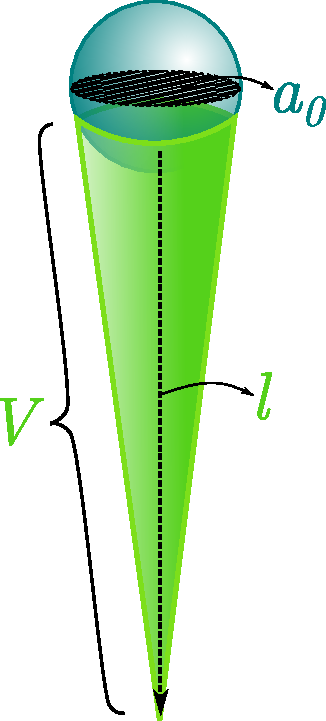
\includegraphics[width=2cm]{imagens/introducao/param_empacotamento}
		\caption{Ilustração do parâmetro de empacotamento}
		\label{fig:param_empacotamento}
	\end{figure}
	
	Esse parâmetro pode ser visualizado como uma comparação entre as áreas das bases de um cilindro, sendo uma dada por \({V}/{l}\) e a outra por \(a_0\). Quando o termo hidrofóbico é pequeno, temos praticamente um cone, e valores de \(P\) menores que \(\sfrac{1}{3}\). Como a região polar é muito grande, a estrutura de autoassociação necessariamente possuirá uma curvatura alta, o que resulta em micelas esféricas. Seguindo esse raciocínio, tanto aumentando a contribuição hidrofóbica quanto diminuindo a contribuição hidrofílica, é possível obter valores de \(\sfrac{1}{3} \leq P < \sfrac{1}{2}\). Nesse momento, são formadas micelas gigantes. Quando as contribuições das duas regiões são equivalentes, (\(P = 1\)), as moléculas de surfactante possuem um formato cilíndrico, sem curvatura. Nessa situação, são formadas estruturas de curvatura zero, como lamelas. Se a contribuição da parte hidrofóbica for muito grande, são formados agregados com grande curvatura, mas de maneira oposta à original são formadas micelas esféricas reversas.
	
	% todo: inserir uma figura com os Ps e as estruturas de autoassociação.
	
	É possível controlar a estrutura de autoassociação controlando-se os parâmetros de \(P\). A adição de um sal inorgânico a um surfactante iônico, por exemplo, blinda as cargas da superfície micelar, diminuindo \(a_0\). Isso diminui a \cmc{} de surfactantes iônicos e, com a adição de sal suficiente, pode causar a transição para micelas cilíndricas, ou até gigantes.
	
	De maneira similar, o aumento da cadeia hidrofóbica (\(l\)) de um surfactante induz a micelização em concentrações menores (diminui a \cmc). Surfactantes com duas caudas, por exemplo, sequer formam micelas esféricas, partindo diretamente para sistemas lamelares em solução. Uma alteração de \(V\) pode ser realizada tanto com o aumento do comprimento da cauda do surfactante, como também com a adição de moléculas apolares, como hidrocarbonetos, que também induzem a micelização. É importante ressaltar que o parâmetro de empacotamento se refere somente à estrutura do surfactante, mas é necessário também considerar o contexto químico do sistema, que pode alterar os parâmetros, se comparados com um surfactante isolado.
	ltando em estruturas diferentes. 
	
	O sistema mais bem descrito na literatura para a formação de micelas gigantes é uma mistura de um surfactante catiônico, como brometo de hexadeciltrimetilamônio (\CTAB) com salicilato de sódio, NaSal. O íon \Sal{} consegue se inserir na superfície micelar, por ser planar, possuir uma região hidrofóbica e carga oposta ao surfactante, e assim diminui \(a_0\) (\ref{fig:interacao_nasal_ctab}). Além disso, as interações cátion-\(\pi\) entre o surfactante e o anel aromático e as interações das partes polares da molécula de salicilato reforçam o posicionamento da molécula na paliçada micelar.
	
	\begin{figure}[H]
		\centering
		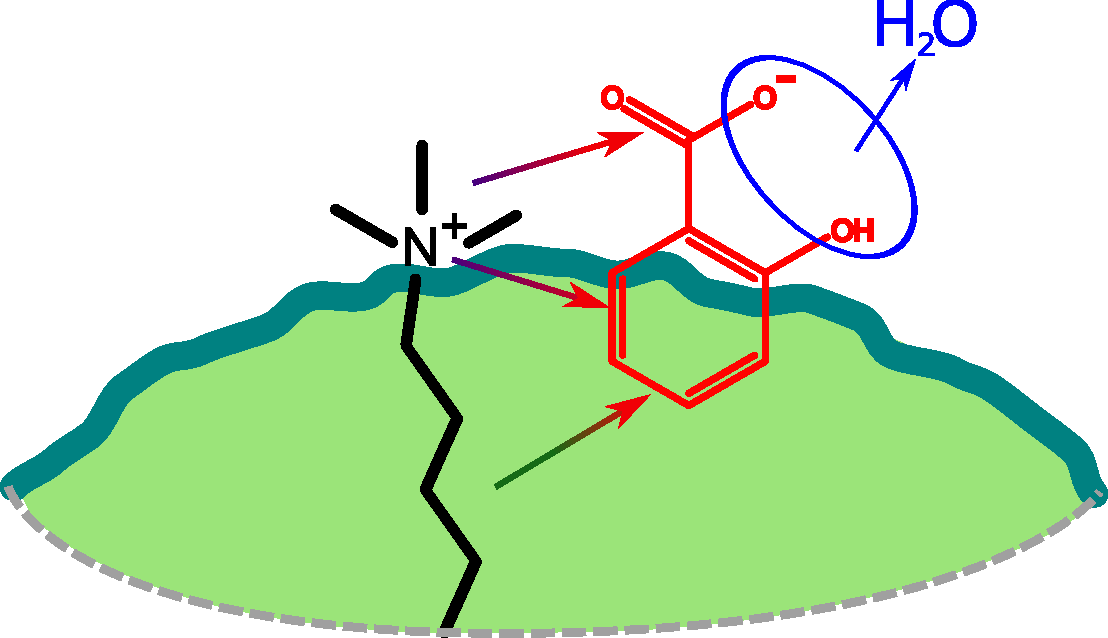
\includegraphics[width=5cm]{imagens/introducao/interacao_nasal_ctab}
		\caption{Interação da molécula de salicilato com um surfactante catiônico e com o solvente}
		\label{fig:interacao_nasal_ctab}
	\end{figure}
	
	Concentrações pequenas, tanto de surfactante quanto de NaSal são capazes de induzir o crescimento micelar, devido à grande afinidade que o salicilato possui pela paliçada. O sistema 100 \mM{} de CTAB e 100 \mM{} de NaSal forma uma solução bastante viscosa, porém uma solução 100 \mM{} de CTAB e 100 \mM{} de NaCl é completamente fluída, devido à baixa afinidade do íon Cl\textsuperscript{-} pela superfície micelar.
	

	
	
	O solvente, como já informado, possui uma papel muito importante na formação de estruturas de autoassociação. Por exemplo, é necessário que exista uma penalidade entrópica da solvatação do surfactante suficientemente grande para que a associação ocorra. Essa penalidade é bastante alta em água, mas muito pequena em solventes como hexano. Apesar de sua importância, não há muitos estudos sobre como o solvente afeta a formação de micelas gigantes. Geralmente, os estudos são feitos em algum solvente puro. Neste trabalho, será estudado o papel de misturas binárias líquidas de água com outro componente na formação de micelas gigantes de NaSal e surfactantes catiônicos.
	
	% todo: achar como é o nome dessa penalidade e colocar alguns exemplos.
	
	Uma descrição mais completa sobre micelas gigantes se encontra no capítulo \ref{chap:micelas_gigantes}.
	
	% todo: pensar sobre o que mais eu posso colocar nesta introdução.
	
	\chapter{Inspirações para o projeto}
	%\section{Inspirações para o projeto}
		\section{Estudos de Hoffmann sobre lamelas e micelas}
		%\subsection{Estudos de Hoffmann sobre lamelas e micelas}
		Hoffmann possui extensa experiência no campo de coloides, possuindo vários artigos importantes sobre micelas gigantes e outras estruturas de autoassociação.
		% X, Y: \cite{Grabner2014, Song2008a}
		
		Em [X, Y], Hoffmann observou que a formação de lamelas não era afetada pela adição de alguns aditivos ao solvente, porém a distância interlamelar aumentava significativamente. A interpretação de Hoffmann para o intumescimento se baseou no índice de refração (\(n\)) do surfactante e do solvente. Quando a concentração de glicerina em água atinge 60\% v/v, o índice de refração do solvente \(n_s\) e do agregado \(n_{ag}\) se tornam iguais. Nessa situação, a atração interlamelar diminui muito, pois a constante de Hamaker, proporcional à diferença desses índices de refração, se torna próxima de zero. Com a atração interlamelar anulada, as forças repulsivas de ondulação das lamelas conseguem separá-las, intumescendo o sistema.
		
		Hoffmann observou o mesmo comportamento para outros sistemas. Os sistemas estudados foram: diacilfosfatidilcolina com glicerina, 1,3-butanodiol, 1,2-propanodiol [X], uma mistura de 5\% de um surfactante não iônico Genapol 070 (LA070) com 50\mM{} de octanol em DMSO, glicerina e sacarose, e lecitina com glicerol [Y].
		
		% Grabner: diacylphosphocholine: glycerol, 1,3-butyleneglycol, 1,2-propyleneglycol, 
		% Song: 5% Non-Ionic Surfactant Genapol 070 (LA070) with 50mM octanol in DMSO/water mixtures and glycerol/water, sucrose (household sugar)/water.
		%       phospholips, lecithin: glycerol, dimethylsulfoxide, sugar(sucrose)
		%       Lecithing: glycerol
		
		% todo: garantir a consistência destes termos ns nag
		% todo: colocar uma lista de sistemas que o Hoffmann observou, para MG
		
		Posteriormente, Hoffmann estudou o efeito do solvente, utilizando glicerina, porém em micelas gigantes de \CTAB{} e NaSal. Observaram que havia uma grande diminuição na viscosidade dos dois picos de viscosidade, mas a região central, de mínimo de viscosidade, era pouco afetada. Nas regiões afetadas, a relaxação micelar ocorre principalmente por meio da reptação, e como a atração intermicelar se torna menor, devido à constante de Hamaker ser próxima de zero, as micelas conseguem reptar mais rapidamente, diminuindo a viscosidade. Na região central, onde o mecanismo principal é a quebra e recombinação, a atração intermicelar é pouco importante, portanto a viscosidade é pouco afetada. Maiores explicações para esse fenômeno podem ser encontradas na seção \ref{sec:efeito_solvente}.
		
		Estudos posteriores foram realizados por Abdel-Rahem, onde foi estudado o efeito do 1,3-butanodiol. Observou-se a concentração de 1,3-butanodiol necessário para resultar numa queda de viscosidade é muito menor que glicerina, nas mesmas condições de índice de refração. Isso informa que considerar somente as interações intermicelares não é suficiente para explicar o efeito do aditivo. O autor levanta a hipótese que há um efeito adicional que está alterando o comportamento, a constante dielétrica, que afeta as interações eletrostáticas no meio. Ambos os parâmetros afetam os mecanismos de relaxação estrutural das micelas, alterando os tempos de relaxação e, consequentemente, as viscosidades.
		% todo: completar os detalhes aqui
		
		Com base nesses estudos prévios, iniciou-se este trabalho de doutorado, que observou o efeito do solvente em soluções de micelas gigantes, atentando-se à parâmetros do solvente, como o índice de refração e constante dielétrica. Outros fatores foram propostos, como o parâmetro de Gordon, relacionado à estruturação do solvente, e com o efeito interfacial dos aditivos nas micelas.
		
		\section{Estudos de Pedersen sobre cinética}
		%\subsection{Estudos de Pedersen sobre cinética}

		% todo: colocar a seção onde eu cito os trabalhos de itc
		
		Durante os estudos deste trabalho, notou-se que haviam resultados de titulações de calorimetria isotérmica que indicavam que poderiam existir dois processos ocorrendo em cada injeção, devido à existência de dois picos. A cinética desse processo era bastante longa. Além disso, esses processos cinéticos lentos ocorriam na região de formação de micelas gigantes. Começou-se a estudar técnicas para a determinação da cinética de crescimento.
		
		Pedersen, em uma série de artigos, observou o crescimento de micelas alongadas utilizando espalhamento de raios-X em baixos ângulos, resolvido no tempo. Para iniciar o crescimento das micelas, foi utilizado um aparato de \emph{stopped-flow}, onde duas soluções, que não continham micelas gigantes, eram misturadas e, após o equilíbrio, as micelas eram formadas.
		
		Em paralelo, observou-se que a fluorescência do salicilato se alterava dependendo da concentração de surfactante no meio. Como será mostrado, a fluorescência é dependente da inserção do salicilato na superfície micelar. Caso esse processo de inserção e crescimento fosse lento o suficiente, seria possível observá-lo por fluorescência resolvida no tempo, realizando um paralelo com os estudos de Pedersen.
		
		Por essas razões, escolheu-se estudar a cinética de crescimento de micelas de \TTAB{} e NaSal, tanto por SAXS resolvido no tempo como por fluorescência resolvida no tempo.
		
	\chapter{Objetivos}
		Os objetivos deste projeto são:
		
		\begin{itemize}[noitemsep]
			\item Estudar como o solvente afeta a reologia de micelas gigantes de \CTAB{} e NaSal.
				\begin{itemize}[noitemsep]
					\item Variar a concentração de NaSal e observar como a viscosidade no repouso, \(\eta_0\), se comporta à medida que mais aditivo é adicionado à água.
						\begin{itemize}[noitemsep]
							\item Aditivos: Glicerina, sacarose, dimetilsulfóxido, 1,3-butanodiol, ureia.
							\item Concentrações: 0-60\% \(m_{\mathrm{aditivo}}/\left(m_{\mathrm{aditivo}}+m_{\mathrm{água}}\right)\), dependendo do aditivo.
						\end{itemize}
					\item Utilizar a teoria vigente na literatura para explicar o comportamento de \(\eta_0\).
					\item Propor novos fatores para complementar a teoria vigente, caso seja necessário.
				\end{itemize}
			\item Estudar como o solvente afeta a formação de micelas gigantes de \TTAB{} e NaSal, através de calorimetria de titulação isotérmica. Os aditivos são os mesmos estudados para reologia.
				\begin{itemize}[noitemsep]
					\item Titular \TTAB{} em NaSal 1,5\mM{} em soluções com concentrações crescentes de aditivo em água.
					\item Titular \TTAB{} nas mesmas misturas binárias.
					\item Comparar os resultados calorimétricos entre si e correlacioná-los com as propriedades do solvente.
					\item Comparar os resultados calorimétricos com os resultados reológicos
				\end{itemize}
			\item Estudar a cinética de crescimento de micelas gigantes através de:
				\begin{itemize}[noitemsep]
					\item Espalhamento de raios-X em baixos ângulos resolvido no tempo. Extrair informações de tamanho pelo ajuste de um modelo apropriado.
					\item Fluorescência de NaSal resolvido no tempo. Extrair informações a partir da taxa de decaimento/crescimento de fluorescência.
				\end{itemize}
			\item Comparar os resultados de cinética com as informações disponíveis na literatura.
		\end{itemize}
	